\section{Monday 09/09/2024}
I also did not attend today so these are slide notes
\subsection{Nonlinear Programming Basic Concepts}
\subsubsection{Nonlinear problem formulation}
\begin{equation}
  \begin{aligned}
    \min_x f(\textbf{x}) \\
    \text{s.t. } h(\textbf{x}) = 0 \\
    g(\textbf{x}) \leq \textbf{0}
  \end{aligned}
\end{equation}
where $f : \mathbb{R}^n \to  \mathbb{R}, h : \mathbb{R}^n \to \mathbb{R}^{m_1}, \text{ and } g : \mathbb{R}^n \to \mathbb{R}^{m_2} $


\begin{itemize}
  \item Objective function, cost function, disutility function
  \item Inequality constraints, non-negativity constraints
  \item Equality constraints
  \item Feasible region, feasible solution
  \item Optimal solution, minimal solution
  \item Unconstrained problems
\end{itemize}

\subsubsection{Global and local solutions definitions}
Let $\Omega := {\textbf{x} : g(\textbf{x} \leq \textbf{0}, h(\textbf{x} = \textbf{0}))}$
\\ \\ 
\framebox[\linewidth]{
    \begin{minipage}{\dimexpr\linewidth-2\fboxsep-2\fboxrule\relax}
        A feasible solution $\textbf{x}^* \in \Omega$ is said to be globally minimal if and only if $f(\textbf{x}^*) \leq f(\textbf{x}) \forall \textbf{x} \in \Omega$
    \end{minipage}
}
\\ \\ 
\framebox[\linewidth]{
    \begin{minipage}{\dimexpr\linewidth-2\fboxsep-2\fboxrule\relax}
        A feasible solution $\textbf{x}^* \in \Omega$ is said to be locally minimal if and only if $f(\textbf{x}^*) \leq f(\textbf{x}) \forall \textbf{x} \in \Omega \cap N(\textbf{x}^*, \epsilon)$ for some $\epsilon > 0 $. Here, $N(\textbf{x}^*, \epsilon) = \{\textbf{x} : ||\textbf{x}^* - \textbf{x} \leq \epsilon||\}$
    \end{minipage}
}
In other words, a global solution is global if it is the minimum of all values in the set. It is locally minimal if it is less than all points in a certain radius defined arbitarily by $\epsilon$.
\subsection{Necessary conditions of optimality}
\subsubsection{Gradients}
Consider a function $f \mathbb{R}^n \to \mathbb{R}$, then the gradient of $f$ is given as 

\begin{align}
  \nabla f(\textbf{x}) := 
  \begin{bmatrix}
     \frac{d f(\textbf{x})}{d x_1} \\ 
     \frac{d f(\textbf{x})}{d x_2} \\ 
     \vdots \\
     \frac{d f(\textbf{x})}{d x_n}
  \end{bmatrix}
\end{align}

Finding gradient of function $f(x_1, x_2) = 0.5x_1^2 + 0.5x_2^2$ at (1,-1)
\begin{gather}
  \frac{d f(\textbf{x})}{d x_1} = x_1 \\
  \frac{d f(\textbf{x})}{d x_2} = x_2
\end{gather}

\begin{align}
  \nabla f(\textbf{x}) = 
  \begin{bmatrix}
    1 \\
    -1
  \end{bmatrix}
\end{align}

\subsubsection{Examples}
a. 
\begin{align}
  \nabla 2 x_1^2 + 2 x_2^2 = 
  \begin{bmatrix}
     4x_1 \\
     4x_2
  \end{bmatrix}
\end{align}
Solving for $\nabla f = 0$,
\begin{align} 
  \textbf{x}^* = 
  \begin{bmatrix}
    0 \\
    0
  \end{bmatrix}
\end{align}
\begin{figure}[htbp]
  \centerline{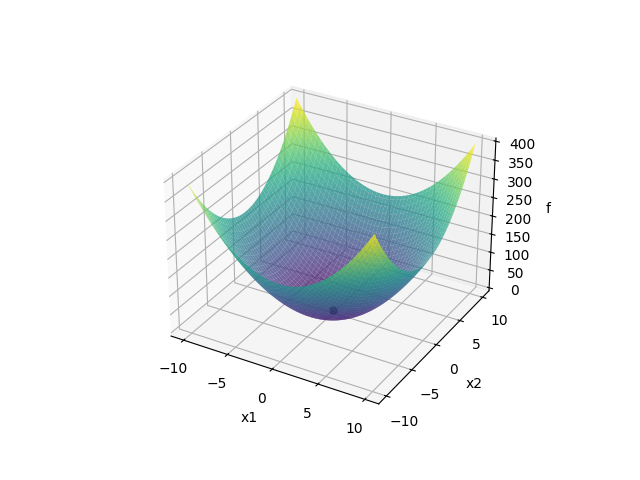
\includegraphics[width=0.75\textwidth]{images/gradient_ex1.png}}
  \caption{Graph of $2 x_1^2 + 2 x_1^2$ with solution at $(x_1,x_2) = (0,0)$}
  \label{fig:gradient_ex1}
\end{figure}
\\ \\ 
b. 
\begin{equation}
  \frac{d \sin(x)}{d x} = \cos(x) 
\end{equation}
Solution to this problem is the curve $\cos(x)$

\begin{figure}[htbp]
  \centerline{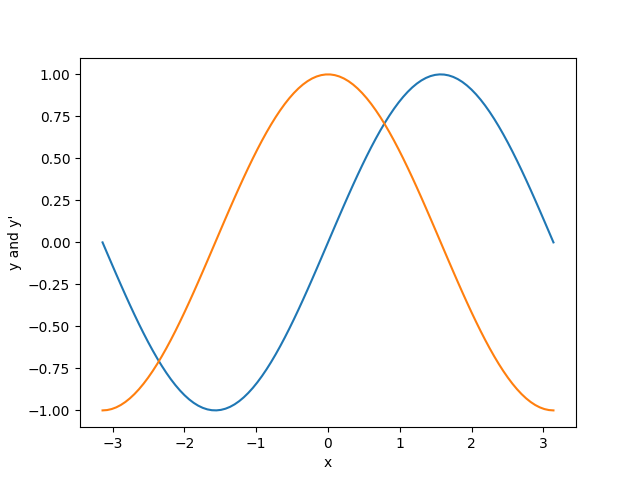
\includegraphics[width=0.75\textwidth]{images/gradient_ex2.png}}
  \caption{Graph of sin(x) and the solution cos(x)}
  \label{fig:gradient_ex2}
\end{figure}

c. 
\begin{equation}
  \frac{d x^3}{d x} = 3x^2 
\end{equation}

Solution to this problem is the curve $3x^2$
\begin{figure}[htbp]
  \centerline{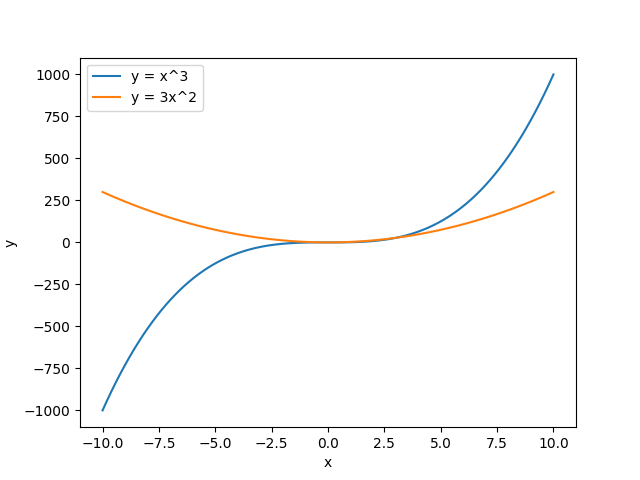
\includegraphics[width=0.75\textwidth]{images/gradient_ex3.png}}
  \caption{Graph of $x^3$ and it's solution $3x^2$}
  \label{fig:gradient_ex3}
\end{figure}

d. 
$(x-3)(x^2-1)(x+2)$ is already in it's factored form so with product rule:
\begin{gather}
  \nabla f = 4x^3 - 3x^2 - 14x + 1
\end{gather}
\begin{itemize}
  \item x = -1.5
  \item x = 2
  \item x = 0
\end{itemize}  

\begin{figure}[htbp]
  \centerline{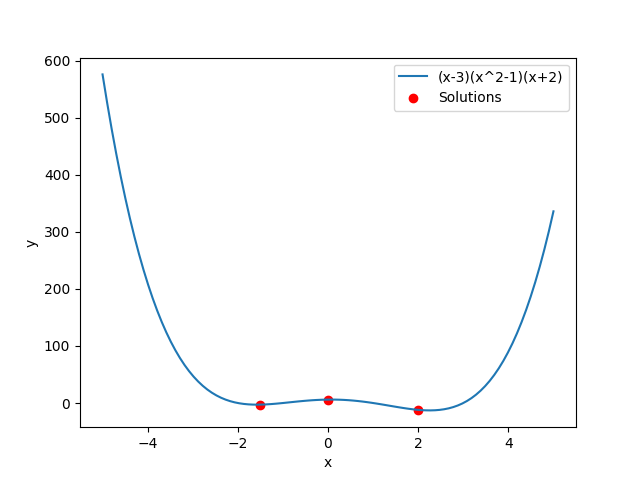
\includegraphics[width=0.75\textwidth]{images/gradient_ex4.png}}
  \caption{Graph of $(x-3)(x^2-1)(x+2)$ and it's solutions $x = 0,-1.5,2$}
  \label{fig:gradient_ex4}
\end{figure}

\section{Wednesday 09/11/2024}
\subsection{Nonlinear programming Part II}
\subsubsection{Problem formulation}

\begin{equation}
  \begin{aligned}
    \min_x f(x) \\
    s.t. g(x) \leq 0
  \end{aligned}
\end{equation}

Now there is a constraint on the problem
\subsubsection{Gradient descent intro}
Dropping a coin into a bowl will cause the coin to travel in the direction of the negative gradient until it reaches $\nabla f = 0$
\begin{figure}[htbp]
  \centerline{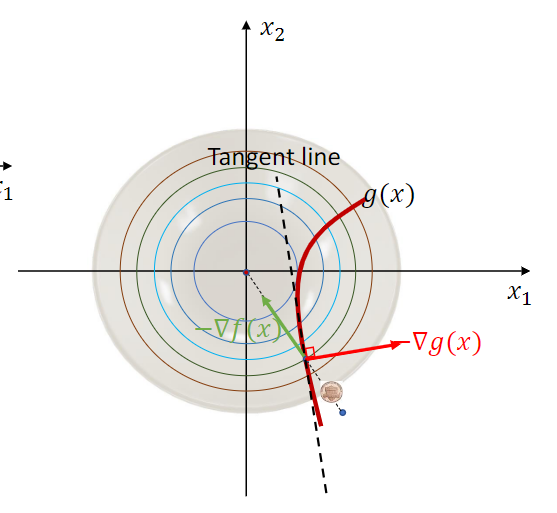
\includegraphics[width=0.75\textwidth]{images/gradient_bowl.png}}
  \caption{A coin traveling in the direction of $-\nabla$ to reach the bottom of the bowl}
  \label{fig:gradient_bowl}
\end{figure}

\begin{equation}
  f(x+\delta d) - f(x) = \left\langle \nabla f(x), \delta d \right\rangle  + 0(\delta^2) = \left\langle \nabla f(x), \delta d \right\rangle
\end{equation}
In the event that $\langle \nabla f(x), \delta d  \rangle < 0$, The step is in a direction that is away from the gradient. It also implies that the gradient is not zero at this point.
\\ \\ 
We can also introduce a constraint function $g(x)$ present in Figure \ref{fig:gradient_bowl} that defines the section (or in the figure's case, a line) that the function $f$ is feasible on. With the introduction of this constraint, the coin can only travel along the path of the constraint $g$. For the solution to be optimal in the context of the function $f$ subject to the constraint $g$, we would need to reach the point where $\nabla f(x^*) + \gamma \nabla g(x^*) = 0 $, where $\gamma = \frac{\| \nabla f \|}{\| \nabla g \|}$

\section{Friday 09/13/2024}
\subsection{Review}
\subsubsection{What is an Inner Product}
An inner product defined as:
\begin{equation}
  \langle u, v \rangle
\end{equation}
is a generalization of the dot product, it effectively gives the answer to the question: How much of one vector is in the direction of the other vector?

\subsubsection{Understanding $g(x^*)=0$}
If $g(x^*) \leq 0 $, then the constraint is being obeyed. The constraint is not obeyed otherwise.
\\ \\
Taking the equation,
\begin{equation}
  g(x^* + \delta d) = \delta \langle \nabla g(x^*), d \rangle - \epsilon
\end{equation}
The step size $\delta$can be moved, and as long as that term is less than zero and does not breach the feasible region.
\\ \\ 
This implies that for a solution to be optimal, $g(x^*) = 0$ must be true, (the converse does not hold).
\subsection{Gradient bowl}
\subsubsection{Adding another constraint}
\begin{figure}[htbp]
  \centerline{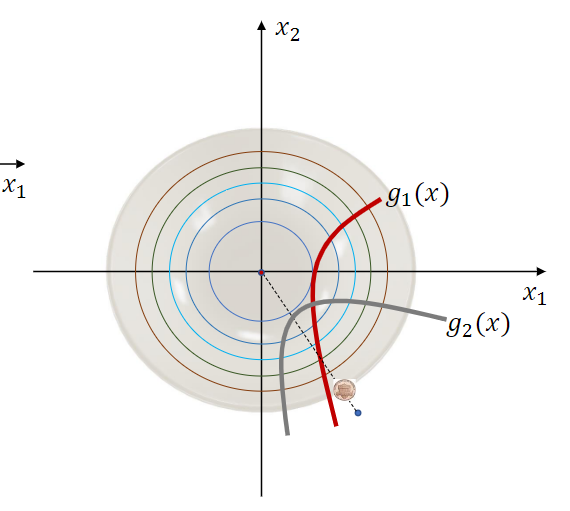
\includegraphics[width=0.50\textwidth]{images/gradient_bowl_cons2.png}}
  \caption{Image of the bowl with a second constraint}
  \label{fig:gradient_bowl_cons2}
\end{figure}

We want to walk opposite of the direction of $\nabla f$ while still walking perpendicular to the gradient of the constraint.
\begin{equation}
  \begin{aligned}
    \min f(x) \\
    s.t. g_1(x) \leq 0 \\
    g_2(x) \leq 0
  \end{aligned}
\end{equation}

A cone is a collection of rays that start from a certain point.
\\ \\ 
In order to find the set of directions we can walk along that will be both improving the objective function while staying in the feasible region, we need to find the intersection of the halfspaces created by each. 
\begin{itemize}
  \item The feasible region based off of $g_1$ is the halfspace created by the set $\{x | \nabla g_1(x) \leq 0 \}$.
  \item The feasible region based off of $g_2$ is the halfspace created by the set $\{x | \nabla g_2(x) \leq 0 \}$.
  \item The "improving" region based off of $f$ is the halfspace created by the set $\{ x | \nabla f(x) \leq 0 \}$.
\end{itemize}
The intersection of these sets is the cone of all possible directions that would result in an improvement to the function while obeying the constraints.

\begin{figure}[htbp]
  \centerline{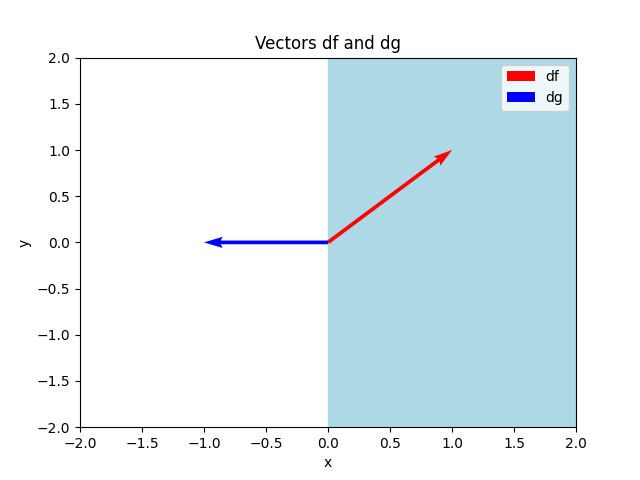
\includegraphics[width=0.75\textwidth]{images/walkable_region.png}}
  \caption{Depicting the walkable region as the intersection between the three regions}
  \label{fig:walkable_region}
\end{figure}

\subsubsection{Finding optimality conditions}
For two constraints $g_1$ and $g_2$, the solution $x^*$ is optimal if 
\begin{equation}
  \nabla f(x^*) + \gamma_1 \nabla g_1(x^*) + \gamma_2 \nabla g_2(x^*) = 0
\end{equation}